As described in the introduction, we infer the polynomial decay under $H$ from exponential decay of some induced return map $H_A$, where returns to $A$ experience `strong' hyperbolic behaviour. The natural choice for $A$, following the work of section \ref{sec:Hmixing}, is the set $\sigma$. We begin by proving the Bernoulli property for $H_\sigma$.

\subsection{Bernoulli property}

\begin{prop}
\label{prop:HsigmaBernoulli}
The return map $H_\sigma$ is Bernoulli with respect to the probability measure $\mu_\sigma = \mu(\sigma)^{-1} \mu $.
\end{prop}

We will show the conditions \textbf{(KS1-3)} and \textbf{(MR)}; the result then follows from Theorem \ref{thm:katok-strelcyn}.

\begin{lemma}
\label{lemma:HsigmaKatokStrelcyn}
The return map $H_\sigma$ satisfies \textbf{(KS1-3)}.
\end{lemma}

\begin{proof}
Starting with \textbf{(KS1)} we follow a similar approach to \cite{springham_polynomial_2014}, their Lemma 4.1. We show that there exists $a,C_1>0$ s.t. $\forall \, \epsilon>0$, $\mu_\sigma(B_\varepsilon(S)) \leq C_1 \varepsilon^a$ for $S = \mathcal{S} \cap \sigma_{1a}$; the argument for the rest of $\mathcal{S}$ is similar and the result then follows by taking a larger $C_1$. Recall the line segments $\mathcal{L}_k$ from ($\dagger$) which for $k \geq 3$ terminate on the points $\left( 0 , (k+1)/(4k+2) \right)$ and $\left( 1/(4k-2) , (k-1)/(4k-2) \right)$ on the line $\mathcal{L}: y= 1/4 -x/2$. Let $P(\varepsilon)$ denote the parallelogram in $\sigma_{1a}$ of width $2\sqrt{\varepsilon}$, height $\sqrt{\varepsilon}$, with sides aligned with $x=0$ and $\mathcal{L}$ (see Figure \ref{fig:sigma1a}). For small $\varepsilon$, $P(\varepsilon)$ contains all line segments $\mathcal{L}_k$ where $2\sqrt{\varepsilon} \geq 1/(4k-2)$, i.e. $k \geq k_0 = \lceil 1/(8\sqrt{\varepsilon}) + 1/2 \rceil$, with
\[ \mu(B_\varepsilon(P(\varepsilon))) = (2\sqrt{\varepsilon} + 2\varepsilon )(\sqrt{\varepsilon} + 2\varepsilon) = 2\varepsilon + 6 \varepsilon^{3/2} + 4\varepsilon^2 < 12\varepsilon. \]
The ball $B_\varepsilon(P(\varepsilon))$ then covers all of $B_\varepsilon(S)$ except the collection $\mathcal{L}_k$, $4 \leq k \leq k_0-1$ and the seven line segments $L_j$ which terminate on $y=2x$. The measure of the ball around these latter line segments satisfies
\[ \mu(B_\varepsilon(\cup_j L_j)) \leq 14 \, \varepsilon \left(\max_j |L_j| + 2\varepsilon \right) < c_1 \varepsilon  \]
for some finite $c_1$, so it remains to estimate $ \sum_{k=4}^{k_0-1} \mu(B_\varepsilon(\mathcal{L}_k))$. We can calculate
\begin{equation}
    \label{eq:Lklength}
    |\mathcal{L}_k| = \sqrt{ \left( \frac{1}{4k-2} \right)^2 + \left( \frac{k+1}{4k+2} - \frac{k-1}{4k-2} \right)^2 } = \sqrt{\frac{8k^2 + 4k+1}{4(4k^2-1)^2 }} < \frac{1}{k} 
\end{equation}
so that
\[ \sum_{k=4}^{k_0-1} \mu(B_\varepsilon(\mathcal{L}_k)) < 2\varepsilon \sum_{k=4}^{k_0-1} \frac{1}{k} + 2\varepsilon < 4\varepsilon^2k_0 + 2\varepsilon \log k_0 < c_2 \varepsilon^a \]
for some $0<a<1$, $c_2>0$ since $k_0 < \varepsilon^{-1/2}$ and there exists finite $c$ such that $c \, \varepsilon^a> \varepsilon \log \frac{1}{\varepsilon}$ for any $0<a<1$.

Since $H_\sigma$ is piecewise linear, condition \textbf{(KS2)} follows trivially and we move onto \textbf{(KS3)}. Existence of Lyapunov exponents almost everywhere follows from Oseledets' theorem \cite{oseledets_multiplicative_1968} provided that $\max \{\log\|DH_\sigma\| ,0 \}$ is integrable. This follows from the fact that if $z \in \sigma$ has return time $R(z;H,\sigma) =k$, then the Jacobian of $H_\sigma$ at $z$ satisfies $\| DH_\sigma \| \leq c_1 k$ for some finite $c_1>0$, and that the measure of the sets $\{ z \in \sigma \, | \, R(z;H,\sigma) =k \}$ are of order $k^{-3}$. That these Lyapunov exponents are non-zero follows from Lemmas \ref{lemma:itineraries}, \ref{lemma:cone} and an argument similar to that given for $H$ in section \ref{sec:OTMhyp}.

\begin{lemma}
\label{lemma:HsigmaMR}
The return map $H_\sigma$ satisfies \textbf{\textbf{(MR)}}.
\end{lemma}

For a.e $z \in \sigma$, local manifolds $\gamma_u(z)$, $\gamma_s(z)$ under $H_\sigma$ align with those of $H$. Note that $H_\sigma$ does not immediately inherit \textbf{(MR)} from $H$ as while successive images of local manifolds under $H$ contain $h$-segments and $v$-segments, these segments may not lie in the successive images under $H_\sigma$.

\begin{figure}
    \centering
    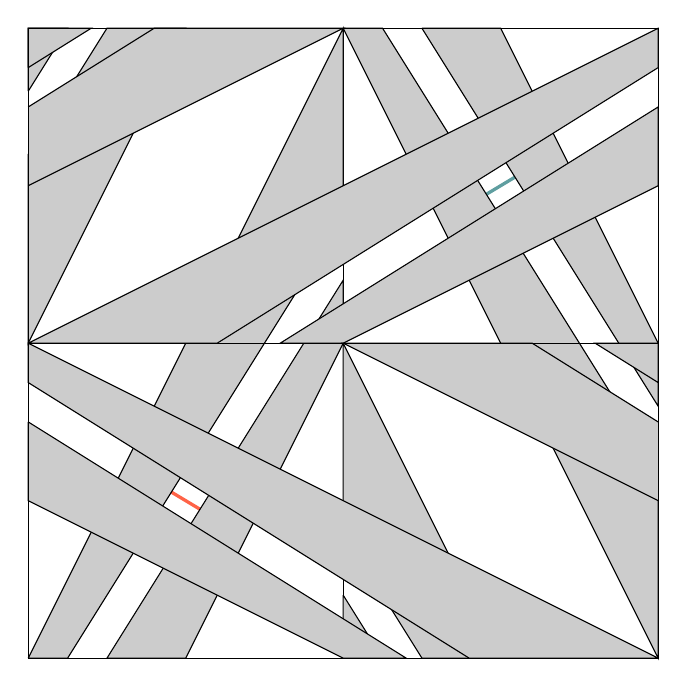
\begin{tikzpicture}[scale=0.8]
    
        
    \definecolor{tomato}{RGB}{255, 99, 71}
    \definecolor{teal}{RGB}{95, 158, 160} 
    
    \draw (5,0) -- (5,10);

    \draw[very thick, tomato] (2,2.8) -- (3,2.2);
    
    \draw[very thick, teal] (10-2,2.8+5) -- (10-3,2.2+5);

    \filldraw[fill=gray!40] (0,8) -- (10/8,10) -- (2.5,10) -- (0,5) -- (0,8);
      \filldraw[fill=gray!40] (0,9) -- (0,10) -- (10/16,10) -- (0,9);
      \filldraw[fill=gray!40] (0,0) -- (5,10) -- (5,7) -- (10/16,0) -- (0,0);
      \filldraw[fill=gray!40] (10/8,0) -- (2.5,0) -- (5,5) -- (5,6) -- (10/8,0) ;
      \filldraw[fill=gray!40] (5,2) -- (50/8,0) -- (7.5,0) -- (5,5) -- (5,2);
      \filldraw[fill=gray!40] (5,1) -- (5,0) -- (90/16,0) -- (5,1);
      \filldraw[fill=gray!40] (5,10) -- (10,0) -- (10,3) -- (90/16,10) -- (5,10);
      \filldraw[fill=gray!40] (50/8,10) -- (7.5,10) -- (10,5) -- (10,4) -- (50/8,10);

    \filldraw[fill=gray!40] (0,150/16) -- (0,10) -- (1,10) -- (0,150/16);
      \filldraw[fill=gray!40] (0,70/8) -- (2,10) -- (5,10) -- (0,7.5);
      \filldraw[fill=gray!40] (0,5) -- (10,10) -- (10,150/16) -- (3,5) -- (0,5);
      \filldraw[fill=gray!40] (10,70/8) -- (10,7.5) -- (5,5) -- (4,5) -- (10,70/8) ;
   
     \filldraw[fill=gray!40] (10,150/16-5) -- (10,10-5) -- (10-1,10-5) -- (10,150/16-5);
      \filldraw[fill=gray!40] (10,70/8-5) -- (10-2,10-5) -- (10-5,10-5) -- (10,7.5-5);
      \filldraw[fill=gray!40] (10,5-5) -- (0,10-5) -- (0,150/16-5) -- (10-3,5-5) -- (10,5-5);
      \filldraw[fill=gray!40] (0,70/8-5) -- (0,7.5-5) -- (10-5,5-5) -- (10-4,5-5) -- (0,70/8-5) ;   

    \draw (0,5) -- (10,5);
    %  \node at (0.65+5,10-9.5) {$\sigma_2$};
    %  \node at (1.25+5,5) {$\sigma_4$};
    %  \node at (2.5+5,10-2.5) {$\sigma_2$};
    % \node  at (4+5,10-1.5) {$\sigma_4$};
     \draw(0,0) rectangle (10,10);
     
     
     
    \end{tikzpicture}
    \caption{The set $\sigma'$ superimposed on $\sigma$, their intersection left white. A $\mathfrak{h}$-segment (red) and a $\mathfrak{h}'$-segment (blue) are plotted in $\mathcal{R}=\sigma_3 \cap \sigma_2'$ and $\mathcal{R}' = \sigma_2 \cap \sigma_3'$ respectively.}
    \label{fig:frakh}
\end{figure}

Let $\mathcal{R}$ denote the quadrilateral $\sigma_3 \cap \sigma_2'$ and $\mathcal{R}' = \sigma_2 \cap \sigma_3'$. Define a $\mathfrak{h}$-segment as a line segment spanning $\mathcal{R}$ with endpoints on $\partial \sigma_3$. Similarly define a $\mathfrak{h}'$-segment as a line segment spanning $\mathcal{R}'$ with endpoints on $\partial \sigma_2$. Examples are plotted in Figure \ref{fig:frakh}. We will show that there exists $M,N$ such that for all $m \geq M$, $n \geq N$, $H_\sigma^m(\gamma_u(z))$ intersects $H_\sigma^{-n}(\gamma_s(z'))$ in either $\mathcal{R}$ or $\mathcal{R}'$. 

By the remark after Theorem \ref{thm:mixingOTM} we can find some $n_2$ such that $H^{-n_2}(\gamma_s(z'))$ contains a $h$-segment in $\sigma_2'$, which in turn contains a $\mathfrak{h}$-segment in $\mathcal{R}$. As a line segment in $\sigma$, this $\mathfrak{h}$-segment lies in $H_\sigma^{-n_1}(\gamma_s(z'))$ for some $n_1 \leq n_2$. Note that we have a hyperbolic period 2 orbit $(1/4,1/4) \leftrightarrow (3/4,3/4)$ under $H_\sigma$, alternating between $\mathcal{R}$ and $\mathcal{R}'$. Any $\mathfrak{h}$-segment $\Lambda$ contains a point $\zeta$ on the unstable manifold through $(1/4,1/4)$ so $H_\sigma^{-2}(\Lambda)$ contains a point $\zeta'$ on the manifold closer to $(1/4,1/4)$ and extends beyond the boundaries $\partial \sigma_3$ by the expansion of $H_\sigma^{-2}$. Hence $H_\sigma^{-2}(\Lambda)$ contains a $\mathfrak{h}$-segment and by induction so does $H_\sigma^{-2k}(\Lambda)$ for all $k\geq 1$. The odd iterates $H^{-2k+1}(\Lambda)$ similarly span $\mathcal{R}'$ so that
\begin{enumerate}[label={($\vee$)}]
    \item Given arbitrary $z' \in \sigma$, there exists $N$ such that for all $n \geq N$ the image $H_\sigma^{-n}(\gamma_s(z'))$ contains a $\mathfrak{h}$-segment or a $\mathfrak{h}'$-segment.
\end{enumerate}
Define a $v'$-segment as a line segment vertically spanning $\sigma_2 \cap S_4$. Condition \textbf{(MR)} now follows from establishing
\begin{enumerate}[label={($\wedge$)}]
    \item Given arbitrary $z \in \sigma$, there exists $M$ such that for all $m \geq M$ the image $H_\sigma^{m}(\gamma_s(z'))$ contains both a $v$-segment \emph{and} a $v'$-segment.
\end{enumerate}
Recall the quadrilaterals $\varsigma_j \subset \sigma_j$ of points with return time 1 (see Figure \ref{fig:returnTime1}). It follows from the definitions of the $\sigma_j$ that $H(\varsigma_2) \subset \sigma_3$ and $H(\varsigma_3) \subset \sigma_2$. The edges of $\varsigma_3$ on the $A_1,A_2$ boundary map into the lines $x=1/2$, $x=1$, in particular onto the red dashed lines on the boundary of $S_2$ in Figure \ref{fig:HSigma} so that the image of any line segment in $\varsigma_3$ which joins these edges contains a $v'$-segment. A analogous result holds for lines segments traversing $\varsigma_2$ and since this behaviour occurs within the return set $\sigma$ we have that $v$-segments map into $v'$-segments under $H_\sigma$ and vice versa. It follows that $v$(')-segments map into $v$(')-segments under $H_\sigma^2$. It suffices to break into the odd iterates to satisfy the `and' condition ($\wedge$).

By following the steps (M1-3) in the proof of Theorem \ref{thm:mixingOTM} we can find $m_2$ such that $H^{m_2}(\gamma_u(z))$ contains a $v$-segment $\Gamma \subset \sigma_3 \cap S_1$ with $H^{-1}(\Gamma) \subset A_3$, $H^{-2}(\Gamma) \subset A_2$, $H^{-3}(\Gamma) \subset A_1$, $H^{-4}(\Gamma) \subset A_4$. In particular $H^{-1}(\Gamma)$ lies in $H(A_2 \cap H(A_1))$, i.e. outside of $\sigma_2$, so that $\Gamma$ lies in $\sigma_3 \setminus (H(\sigma_2) \cap \sigma_3)$. The set $H(\sigma_2) \cap S_1$ (shown in blue in Figure \ref{fig:HsigmaMR}) is the quadrilateral with corners $(7/68,0)$, $(3/34,0)$, $(27/68,0)$, $(7/17,0)$, which splits $\sigma_3 \cap S_1$ into left and right parts. We assume first that $\Gamma$ lies in the right part, intersecting the line $y=1/2$ at some point $(x_1,1/2)$ with $x_1 \geq 7/17$ and the $A_1,A_2$ boundary $y=1/2-x/2$ at some point $(1-2y_1,y_1)$. These intersections define a line segment $\Gamma_1 \subset \Gamma$, which lies in $A_1$ shown in Figure \ref{fig:HsigmaMR}. Applying $F$ maps $(x_1,1/2)$ to itself (wrapping horizontally around the torus) and maps $(1-2y_1,y_1)$ to $(0,y_1)$. Applying $G$ then leaves $(0,y_1)$ invariant and wraps $(x_1,1/2)$ vertically around the torus to $(x_1, 1/2 + 2x_1) \text{ mod }1 \equiv (x_1,-1/2+2x_1)$. Since $x_1 \geq 7/17$ we have that $-1/2 + 2x_1 \geq 11/34 > 10/24 \geq 1/2 - x_1/2$ so that $(x_1,-1/2+2x_1)$ lies above the line $y=1/2-x/2$. We restrict again to $A_1$, giving $\Gamma_2 \subset H(\Gamma_1)$ with endpoints on $(x_1,-1/2+2x_1)$ and some point $(1-2y_2,y_2)$ on $y=1/2-x/2$. This line meets $y=-1/2+2x$ at $(2/5,3/10)$ so that $y_2 \leq 3/10$ (see Figure \ref{fig:HsigmaMR}). Now $F(\Gamma_2)$ joins $(0,y_2)$ to $(5x_1 -2, 2x_1 - 1/2)$ and so $H(\Gamma_2)$ joins $(0,y_2)$ to $(5x_1-2,12x_1-9/2)$. The set $A_{3,2}^1$ is bounded by the parallel lines $y=7/16 -5x/8$ and $y=3/8 - 5x/8$. Since $y_2<3/8$ and $12x_1-9/2 \geq 15/34 > 109/272 \geq 7/16 - 5(5x_1 -2)/8$ we have that $H(\Gamma_2)$ contains a segment $\Gamma_3$ which traverses $A_{3,2}^1$. The image $H(\Gamma_3)$ then traverses $Q_3$ so that $H^2(\Gamma_3) \subset H^4(\Gamma)$ contains a $v$-segment in $\sigma_3$. Critically we have that $\Gamma_2,\Gamma_3 \subset H(A_1) \subset \sigma$ but $\Gamma_4 \subset H(A_2 \cap H(A_1))$ which is not in $\sigma$. Hence $H_\sigma^3(\Gamma)$ contains a $v$-segment and we can apply the $H_\sigma^2$ result above to show that $H_\sigma^k(\Gamma)$ contains a $v$-segment for all $k \geq 2$. Similar analysis can be applied to $\Gamma$ in the left portion of $\sigma_3 \setminus (H(\sigma_2) \cap \sigma_3)$. It follows that $H_\sigma^k(\Gamma)$ contains a $v'$-segment for all $k \geq 3$, establishing ($\wedge$) with $M=m_1+3$.
\end{proof}
\begin{figure}
    \centering

    \begin{tikzpicture}
    
            
    \definecolor{tomato}{RGB}{255, 99, 71}
    \definecolor{teal}{RGB}{95, 158, 160} 
    
    \node at (-3.5,0) {
  
    \begin{tikzpicture}[scale=1.3]
    \node at (-0.15,350/104) {$y_1$};
    \clip (0,0) rectangle (5,5);
    
    \fill [fill=white] (0,0) -- (2.5,5) -- (5,5) -- (2.5,0) -- (0,0);
    
    \draw (0,5) -- (10,0);
    \draw (0,2.5) -- (5,0);
    
    
    
    \filldraw[fill=gray!80] (0,0) -- (5,10) -- (5,7) -- (10/16,0) -- (0,0);
    \filldraw[fill=gray!80] (10/8,0) -- (2.5,0) -- (5,5) -- (5,6) -- (10/8,0) ;
      
    \filldraw[teal] (70/17,5) -- (70/68,0) -- (30/34,0) -- (270/68,5) -- (70/17,5);
    

    \draw[very thick] (170/52,350/104) -- (4.25,5);
    
    \draw [dashed, thick] (0,350/104) -- (4.25,5);
    

    
    \draw [very thick] (0,350/104) -- (0.8724691416999097,5);
    \draw [very thick] (2.782261032261033,0) -- (4.25,3.5);
    
    \begin{scope}
    \clip (0,5) -- (5,2.5) -- (5,5) -- (0,5);
    \draw [very thick, tomato] (2.782261032261033,0) -- (4.25,3.5);
    \end{scope}
    
    \node at (4.15,4.3) {$\Gamma_1$};
    
    \node at (1.3,3.55) {$F(\Gamma_1)$};
    
    \node at (4.35,3.2) {\color{tomato}$\Gamma_2$\color{black}};


    \draw (0,0) rectangle (5,5);
    \end{tikzpicture}};
    
    
    
    
    \node at (4,0) {
    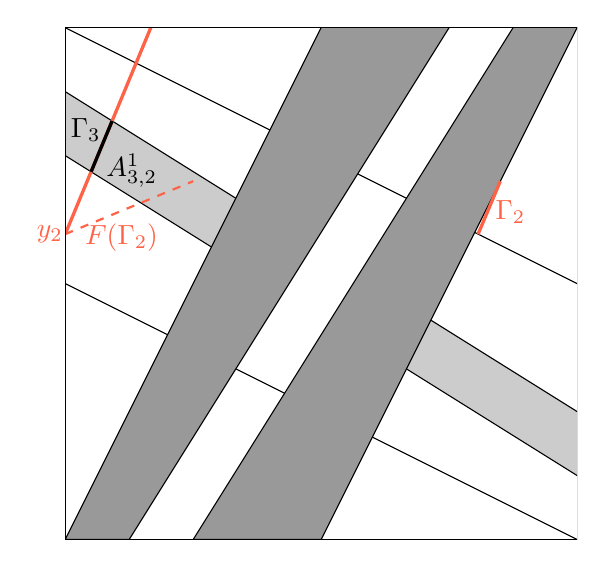
\begin{tikzpicture}[scale=1.3]
    
    \node at (-0.15,2.98323) {\color{tomato}$y_2$\color{black}};
    
    \clip (0,0) rectangle (5,5);

    \filldraw[fill=gray!40] (0,150/16-5) -- (7,0) -- (6,0) -- (0,70/8-5) --(0,150/16-5);

    \fill [fill=white] (0,0) -- (2.5,5) -- (5,5) -- (2.5,0) -- (0,0);
    
    \draw (0,5) -- (10,0);
    \draw (0,2.5) -- (5,0);
    
    
    \filldraw[fill=gray!80] (0,0) -- (5,10) -- (5,7) -- (10/16,0) -- (0,0);
    \filldraw[fill=gray!80] (10/8,0) -- (2.5,0) -- (5,5) -- (5,6) -- (10/8,0) ;
    
    \begin{scope}
    \clip (0,5) -- (5,2.5) -- (5,5) -- (0,5);
    \draw [very thick, tomato] (2.782261032261033,0) -- (4.25,3.5);
    \end{scope}
    
    \draw[dashed, thick, tomato] (0,2.98323) -- (1.25,3.5);
    \draw[very thick, tomato] (0,2.98323) -- (1.25,6);
    
    \draw [very thick] (0.25249,3.59197) -- (0.45807,4.08851);
    
    \node at (0.55,2.95) {\color{tomato}$F(\Gamma_2)$\color{black}};
    
    \node at (0.2,4) {$\Gamma_3$};
    
    \node at (0.65,3.6) {$A_{3,2}^1$};
    
    \node at (4.35,3.2) {\color{tomato}$\Gamma_2$\color{black}};

    \draw (0,0) rectangle (5,5);
    
    \end{tikzpicture}};

    \node at (-1.02,3.45) {$x_1$};
    
      \end{tikzpicture}
    
    
    
        
    \caption{Left: The upper part $\Gamma_1 \subset A_1$ of a $v$-segment in $\sigma_3 \setminus (H(\sigma_2) \cap \sigma_3)$ and its images $F(\Gamma_1)$ (dashed), $H(\Gamma_1) \cap S_1$. Right: A right part $\Gamma_2 \subset A_1$ of $H(\Gamma_1)$ and its images $F(\Gamma_2)$, $H(\Gamma_2) \cap S_1$. This image necessarily contains a line segment $\Gamma_3$ traversing $A_{3,2}^1$.}
    \label{fig:HsigmaMR}
    \end{figure}

\subsection{Invariant cones}
\label{sec:invariantCones}
We now derive specific unstable and stable cone fields for the return map $H_\sigma$, wide enough to ensure invariance \textbf{(H1.1)} yet fine enough to produce tight bounds on expansion factors, vital for verifying \textbf{(H5)}. Define the cones $\mathcal{C}_1,\dots,\mathcal{C}_4$ by
\begin{enumerate}[label={($\mathcal{C}_{\arabic*}$)}]
    \item $3|v_1| \geq |v_2| \geq 7 |v_1|/3$, $v_1v_2>0$,
    \item $5|v_1|/3 \geq |v_2| \geq \varphi |v_1|$, $v_1v_2<0$,
    \item $5|v_1|/3 \geq |v_2| \geq \varphi |v_1|$, $v_1v_2>0$,
    \item $3|v_1| \geq |v_2| \geq 7 |v_1|/3$, $v_1v_2<0$,
\end{enumerate}
and the following stable cones
\begin{enumerate}[label={($\mathcal{C}_{\arabic*}^s$)}]
    \item $|v_1| \geq |v_2|$,
    \item $9/10 \geq v_2/v_1 \geq -8/10$,
    \item $8/10 \geq v_2/v_1 \geq -9/10$,
    \item $|v_1| \geq |v_2|$.
\end{enumerate}

\begin{figure}
    \centering
    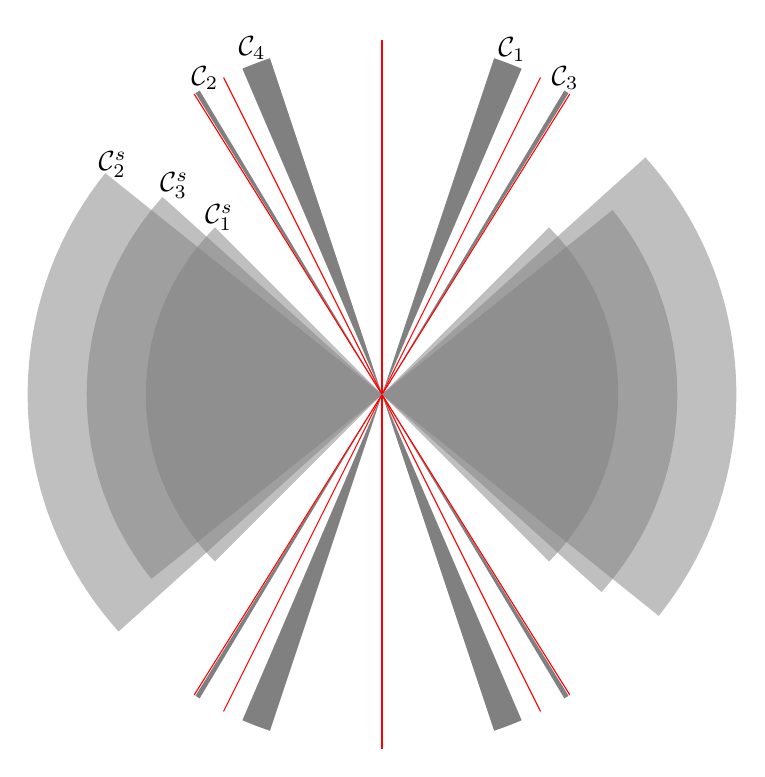
\begin{tikzpicture}[scale=1.5]
    
    \begin{scope}
    \clip (0,0) circle (3cm);
     \fill[gray] (0,0) -- (10,210/13) -- (10,50/3) -- (0,0);
     \fill[gray] (0,0) -- (-10,-210/13) -- (-10,-50/3) -- (0,0);
     \fill[gray] (0,0) -- (-10,210/13) -- (-10,50/3) -- (0,0);
     \fill[gray] (0,0) -- (10,-210/13) -- (10,-50/3) -- (0,0);
     
     \fill[gray] (0,0) -- (10,70/3) -- (10,30) -- (0,0);
     \fill[gray] (0,0) -- (10,-70/3) -- (10,-30) -- (0,0);
     \fill[gray] (0,0) -- (-10,70/3) -- (-10,30) -- (0,0);
     \fill[gray] (0,0) -- (-10,-70/3) -- (-10,-30) -- (0,0);
     
     \fill[gray,opacity=0.5] (0,0) -- (-10,8) -- (-10,-9) -- (0,0);
     \fill[gray,opacity=0.5] (0,0) -- (10,-8) -- (10,9) -- (0,0);
     
     \draw[red] (-10,-80/5) -- (10,80/5);
     \draw[red] (10,-80/5) -- (-10,80/5);
     
     \draw[red] (-10,-20) -- (10,20);
     \draw[red] (10,-20) -- (-10,20);
     
     \draw[red] (0,-10) -- (0,10);
    
     
    \end{scope}
   
    \begin{scope}
    \clip (0,0) circle (2.5cm);
    \fill[gray,opacity=0.5] (0,0) -- (-10,9) -- (-10,-8) -- (0,0);
     \fill[gray,opacity=0.5] (0,0) -- (10,-9) -- (10,8) -- (0,0);
    
    \end{scope}
   
   
   \begin{scope}
    \clip (0,0) circle (2cm);
    \fill[gray,opacity=0.5] (0,0) -- (-10,10) -- (-10,-10) -- (0,0);
     \fill[gray,opacity=0.5] (0,0) -- (10,-10) -- (10,10) -- (0,0);
    \end{scope}
   
   
  \node at (-1.38,1.4+0.1) {$\mathcal{C}_1^s$};
  \node at (-1.76,1.67+0.1) {$\mathcal{C}_3^s$};
  \node at (-2.28,1.85+0.1) {$\mathcal{C}_2^s$};
  
  \node at (-1.5,2.68) {$\mathcal{C}_2$};
    \node at (1.55,2.68) {$\mathcal{C}_3$};
    
    \node at (-1.1,2.93) {$\mathcal{C}_4$};
    \node at (1.1,2.92) {$\mathcal{C}_1$};
  
    
    \end{tikzpicture}
    \caption{Unstable and stable cone fields $\mathcal{C}_j$, $\mathcal{C}_j^s$ over the subsets $\sigma_j \subset \sigma$ for the return map $H_\sigma$. Also shown in red are the gradients of the line segments which make up the boundary $\partial \sigma$ which lie outside of all cone fields.}
    \label{fig:HsigmaCones}
\end{figure}
In the notation of section \ref{sec:outline}, for general $z \in \sigma$ we take $C_z^u = \mathcal{C}_j$ and $C_z^s = \mathcal{C}_j^s$ for $z \in \sigma_j$. These cone fields are plotted in Figure \ref{fig:HsigmaCones}.

\begin{table}[h]
    \centering
    \begin{tabular}{c||c|c|c|c}
         $DH_\sigma$ & $\sigma_1$ & $\sigma_2$ & $\sigma_3$ & $\sigma_4$  \\
         \hline \hline
         $\sigma_1$  & $M_1$ & - & $M_3M_2^k$ & \makecell{$M_4$ \\ $M_4M_2^k$ \\ $M_4M_3^k$} \\
         \hline
         $\sigma_2$  & - & - & \makecell{$M_3$ \\ $M_3M_2$ \\ $M_3M_2^2$} & \makecell{$M_4$ \\ $M_4M_2$ \\ $M_4M_2^2$} \\
         \hline
         $\sigma_3$  & \makecell{$M_1$ \\ $M_1M_3$ \\ $M_1M_3^2$ }& \makecell{$M_2$ \\ $M_2M_3$ \\  $M_2M_3^2$} & - & - \\
         \hline
         $\sigma_4$  & \makecell{$M_1$ \\$M_1M_2^k$ \\ $M_1M_3^k$} & $M_2M_3^k$ & - & $M_4$ \\
    \end{tabular}
    \caption{Possible values of the Jacobian $DH_\sigma$ at $z$ if $z \in \sigma_i$ (rows) and $z' = H_\sigma(z) \in \sigma_j$ (columns). Exponent $k$ takes values in $\mathbb{N}$, dashes are shown if no transition is possible, e.g $H_\sigma(\sigma_1) \cap \sigma_2 = \varnothing$.}
    \label{tab:sigmaTransitions}
\end{table}

\begin{lemma}
\label{lemma:finalReducedCones}
The above cones satisfy $DH_\sigma \, C_z^u \subset C_{z'}^u$ and $DH_\sigma \, C_z^s \supset C_{z'}^s$ for all $z\in \sigma$ where $DH_\sigma$ exists, $z'=H_\sigma(z)$. 
\end{lemma}

\begin{proof}
We begin with the unstable cones. Table \ref{tab:sigmaTransitions} shows the possible values of $DH_\sigma$ at $z$ if $z \in \sigma_i$ and $z' \in \sigma_j$. The calculations for $z' \in \sigma_1,\sigma_4$ are similar to those made in the proof of Lemma \ref{lemma:mappedOTMalignment}, noting that each $\mathcal{C}_j$ is contained within $\mathcal{C}$ and, for example, $M_1M_j^k \mathcal{C} \subset \mathcal{C}_1$ for $j=2,3$, and $k \geq 0$. For $z' \in \sigma_2$ we verify that $M_2M_3^k (-1,3)^T =(-1)^k (-24k+5,-40k-7)^T \in \mathcal{C}_2$ and $M_2M_3^k (-3,7)^T =(-1)^k (60k+11,-100k-15)^T \in \mathcal{C}_2$ for all $k \geq 1$ so that $DH_\sigma \, C_z^u \subset C_{z'}^u$ for $z \in \sigma_4$. For $z \in \sigma_3$ we have $M_2 (3,5)^T = (13,-21)^T \in \mathcal{C}_2$ and $M_2 (13,21)^T = (55,-89)^T \in \mathcal{C}_2$, ensuring invariance in this particular case also, despite $M_2$ being non-hyperbolic. Entirely symmetric calculations can be made for $z' \in \sigma_3$, verifying the result for all unstable cones.

For the stable cones, we remark that taking $C_z^s = \mathcal{C}_1^s$ for all $z \in \sigma $ would satisfy $DH_\sigma \, C_z^s \supset C_{z'}^s$ but since $M_2^{-1} (1,-1)^T = (-1,1)^T$ we would be unable to derive sufficient uniform bounds on expansion factors \textbf{(H1.2)}. The matrix $M_3^{-1}$ exhibits a similar problem so we must slim down the cones $C_z^s$ when $DH_\sigma^{-1} \in \{ M_2^{-1}, M_3^{-1} \}$ which, observing Table \ref{tab:sigmaTransitions}, is for $z \in \sigma_2,\sigma_3$. To remedy this, for such $z$ we slim down the cones $C_z^s$ to $\mathcal{C}_2^s,\mathcal{C}_3^s$ above. As these cones lie in the wider invariant cone $|v_1| \geq |v_2|$, the lemma follows from checking that $DH_\sigma \, C_z^s \supset C_{z'}^s$ for $z \in \sigma_2,\sigma_3$. This can be verified via direct calculations.
\end{proof}



\subsection{Structure of the singularity set}
\label{sec:singSetStructure}
Using the notation of \textbf{(H2)} in section \ref{sec:outline}, let $\mathcal{S}_0 = \cup_j \partial \sigma_j$, the union of $\partial \sigma$ and the red dashed lines in Figure \ref{fig:HSigma}. The set $M = \Omega \setminus \mathcal{S}_0$ is clearly dense in $\Omega$ and $H_\sigma$ is a $C^2$ diffeomorphism from $M\setminus \mathcal{S}_1$ onto $M \setminus \mathcal{S}_{-1}$, being linear on each component. 

The set $\mathcal{S}_0 \cup \mathcal{S}_1$ is the countable union of bounded line segments with the endpoints of each segment terminating on another segment, giving \textbf{(H2.2)}. 

The gradients of the segments in $\mathcal{S}_0$ take values in $\{ \pm 8/5, \pm 2, \infty \}$ which avoid unstable and stable cones $C_z^u$, $C_z^s$ (see Figure \ref{fig:HsigmaCones}). The gradients of singularity curves in $\sigma_1$ and $\sigma_4$ are bounded between -1 and 1 (approaching these limits as we approach the accumulation points) so lie in $\mathcal{C}_1^s,\mathcal{C}_4^s$. The gradients of singularity curves in $\sigma_2$ and $\sigma_3$ are bounded between -11/14 and 11/14 so lie in $\mathcal{C}_2^s,\mathcal{C}_3^s$ since $11/14 < 8/10$. Similar calculations show that the gradients of segments in $\mathcal{S}_{-1}$ lie in unstable cones.

We conclude this section with showing \textbf{(H2.4)}. Condition (\ref{eq:DxbCondition}) can only fail when $\| DH_\sigma \|$ becomes unbounded, i.e. at points $z$ approaching the accumulation points. We consider the case with $z \in A_{4,2}^k$ near $(0,1/4)$, the other cases are similar. Recall Figure \ref{fig:sigma1a} and the lines $\mathcal{L}_k$ from ($\dagger$). We note that $d(z,\mathcal{S}_1)$ is bounded above by the length of the segment joining $z=(x,y)$ to $(x,y_k(x))$ on $\mathcal{L}_k$, which in turn is bounded above by the height of the segment joining $(x,y_k(x))$ to $(x,y_{k-1}(x))$ on $\mathcal{L}_{k-1}$. This height is
\[ y_{k-1}(x) - y_k(x) \leq y_{k-1}\left( \frac{1}{4k-2}\right) - y_k\left( \frac{1}{4k-2} \right) = \frac{1}{2(2k-1)^2} \leq c_1 /k^2  \]
for some constant $c_1>0$. The operator norm of $DH_\sigma$ over $A_{4,2}^k$ satisfies $\| DH_\sigma \| \leq c_2 k$ for some $c_2>0$ so that (\ref{eq:DxbCondition}) holds for some $c>0$ whenever we choose $b>1/2$.

\subsection{One-step expansion}
\label{sec:twoStepExpansionOTM}
We will verify (\ref{eq:oneStep}) for the map $f=H_\sigma^2$, $q=1/2$. We begin with a basic statement on expansion over unstable curves.

\begin{lemma}
\label{lemma:piecewiseApprox}
Let $M$ be the constant Jacobian of $f$ over $W_i$, $V_i =f(W_i)$. Then
\[ \lambda^{-} := \inf_{v\in \mathcal{C}} \frac{\| M v \|}{\|v \|} \leq \frac{|V_i|}{|W_i|} \leq  \sup_{v\in \mathcal{C}} \frac{\| M v \|}{\|v \|} =: \lambda^+. \]
\end{lemma}

\begin{proof}
Given any $\varepsilon>0$, consider a piecewise linear approximation $\hat{W_i}$ to $W_i$ such that
\[ \left| \frac{|V_i|}{|W_i|} - \frac{|\hat{V_i}|}{|\hat{W_i}|}  \right| < \varepsilon \]
where $\hat{V_i} = f(\hat{W_i})$ gives a piecewise approximation for $V_i$. Each of the piecewise components will be line segments aligned with vectors in $\mathcal{C}$ so that their expansion factors will be bounded by $\lambda^\pm$, giving the result.
\end{proof}

We also derive basic inequalities on the length of a given $W_i$.

\begin{lemma}
\label{lemma:componentLength}
Let $\mathcal{L}_0,\mathcal{L}_1$ be the singularity curves on which $W_i$ terminates, write these intersections as $(x_0,y_0)$ and $(x_1,y_1)$. Then
\[ \sqrt{(x_1-x_0)^2 + (y_1-y_0)^2} \leq |W_i| \leq |y_1-y_0|\sqrt{1+\frac{1}{g^2}}\]
where $g = \inf|v_2/v_1|$ over $(v_1,v_2)^T \in \mathcal{C}$. 
\end{lemma}

\begin{proof}
Noting that the lower bound is trivial, we focus on the upper bound. Since $g>0$ for all unstable cones $\mathcal{C}$, the projection of $W_i$ to the $y$-axis is injective. Without loss of generality suppose $y_1>y_0$, then we can parameterise $W_i$ as a curve $(x(y),y)$ for $y_0\leq y \leq y_1$. Now
\begin{equation*}
\begin{split}
    |W_i| &= \int_{y_0}^{y_1} \sqrt{ \left(\frac{\mathrm{d}x}{\mathrm{d}y} \right)^2 + \left(\frac{\mathrm{d}y}{\mathrm{d}y}\right)^2 } \d y \\
    & \leq (y_1-y_0) \sup_{y_0\leq y \leq y_1} \sqrt{1+ \left(\frac{\mathrm{d}x}{\mathrm{d}y}\right)^2}\\
    & \leq (y_1-y_0)  \sqrt{1+ \frac{1}{g^2}}
    \end{split}
\end{equation*}
as tangent vectors $(x'(y),1)^T$ to $W_i$ lie in $\mathcal{C}$. 
\end{proof}

Let $P_1 = \{ (0,1/4), (1/2,1/4), (1/2,3/4), (1,3/4) \}$ denote the accumulation points similar to that of $\sigma_{1a}$, $P_2 = \{ (1/4,1/2), (1/4,1), (3/4,0), (3/4,1/2) \}$ the accumulation points similar to that of $\sigma_{1b}$. Let $\varepsilon$ be small. Given a set $P$, let $B_\varepsilon(P)$ denote the union of the balls $B_\varepsilon(p) \cap \sigma$, centred at $p\in P$ of radius $\varepsilon$. The following describes the images of balls about $P_1 \cup P_2$ under $H_\sigma$.

\begin{lemma}
\label{lemma:accumulationMapping}
Given small $\varepsilon>0$, there exists some $\varepsilon'>0$ such that $H_\sigma(B_\varepsilon(P_1 \cup P_2))$ covers $B_{\varepsilon'}(P_1 \cup P_2)$.
\end{lemma}

\begin{proof}

We describe the covering of $B_{\varepsilon'}((1/2,3/4))$, analysis for the other points in $P_1\cup P_2$ is analogous. For any $\varepsilon>0$, $B_\varepsilon(P_1 \cup P_2)$ contains the sets $A_{4,3}^k$ for all $k \geq k_0$ where $k_0 \in \mathbb{N}$ depends on $\varepsilon$. Each $A_{4,3}^k$ consists of two quadrilaterals, one in the ball around $(1/4,1)$ and the other in the ball around $(1/4,1/2)$. Figure \ref{fig:twoStepA} shows this latter quadrilateral, with corners on the points
\[  r_1 = \left( \frac{k+1}{4k+2}, \frac{k+1}{2k+1}  \right), \quad r_2 = \left(\frac{k-1}{4k-2}, \frac{1}{2}  \right), \quad r_3 = \left(\frac{k}{4k+2}, \frac{1}{2}  \right), \quad r_4 = \left(\frac{k+2}{4k+6}, \frac{k+2}{2k+3}  \right).  \]
Since $DH_\sigma$ is constant on $A_{4,3}^k$, given by the integer valued matrix $M_4M_3^k = (-1)^k \big(\begin{smallmatrix}
  2k+1 & -2k-2\\
  -6k-2 & 6k+5
\end{smallmatrix}\big)$,
its image $H_\sigma\left(A_{4,3}^k\right)$ is given by the quadrilateral with corners given by $M_4M_3^k \, r_j^T \text{ mod }1$. For odd $k$ we can calculate these corners as
\[  r_1'(k) = \left( \frac{1}{2} + \frac{1}{4k+2} , \frac{3}{4} -\frac{5}{8k+4}  \right), \quad r_2'(k) = \left( \frac{1}{2} + \frac{1}{4k-2} , \frac{3}{4} - \frac{5}{8k-4}  \right),\] \[r_3'(k) = \left( \frac{1}{2} , \frac{3}{4} + \frac{1}{8k+4}  \right), \quad r_4'(k) = \left( \frac{1}{2} , \frac{3}{4} + \frac{1}{8k+12}  \right), \]
shown in Figure \ref{fig:twoStepB}. For even $k$ the corners of $A_{4,3}^k$ in the ball around $(1/4,1)$ map into the $r_j'$. Writing this quadrilateral as $Q(k)$, since $r_2'(k+1)$ = $r_1'(k)$ and $r_3'(k+1) = r_4'(k)$ we have that $\cup_{k \geq k_0} Q(k)$ is the polygon with corners $r_2'(k_0)$, $r_3'(k_0)$, and $\lim_{k\to \infty} r_1'(k) = \lim_{k \to \infty} r_4'(k) = (1/2,3/4)$. Noting that $r_3'(k_0) > 3/4$ and $r_2'(k_0)$ lies on the line $y-\frac{3}{4} = -\frac{5}{2}(x-\frac{1}{2})$, there exists $\varepsilon'$ such that $\cup_{k \geq k_0} Q(k)$ covers all points $(x,y) \in B_{\varepsilon'}((1/2,3/4))$ with $y \geq \frac{3}{4} - \frac{5}{2}(x-\frac{1}{2})$. The image $H_\sigma( B_\varepsilon((1,3/4)) \cap A_4 )$ fills the remaining portion of $B_{\varepsilon'}((1/2,3/4))$, since $H_\sigma = H$ on $A_4$, $H(1,3/4) = (1/2,3/4)$, $DH \,(-2,1)^T = (0,-1)^T$, and $DH \,(0,-1)^T = (2,-5)^T$.
\end{proof}

\begin{prop}
\label{prop:simple2step}
Condition (\ref{eq:oneStep}) holds for $H_\sigma^2$ when there exists $\varepsilon>0$ such that $W \cap B_\varepsilon(P_1 \cup P_2) = \varnothing$.
\end{prop}

\begin{proof}

We claim that an unstable curve $W$ of vanishing length, bounded away from the accumulation points, is split into at most 9 components $W_i$ by the singularity set for $H_\sigma^2$. The upper bound follows from analysis of the original singularity set for $H_\sigma$. Let $P_F$ denote the set of fixed points under $H$, $P_F = \{ (0,1/2), (1/2,0), (1/2,1/2), (1,1) \}$. Observing Figure \ref{fig:sigmaSingSet}, if $W \cap B_\varepsilon(P_F) \neq \varnothing$ then $W$ is split by $\mathcal{S}$ into at most 5 components $W_j$, and if $W \cap B_\varepsilon(P_F) = \varnothing$ then the upper bound is 3. We consider these cases separately. 

Take, for example, $W \cap B_\varepsilon((0,1/2)) \neq \varnothing$. Observing Figure \ref{fig:sigma1b}, four of the components $W_j$ map into $A_4'$ under $H_\sigma$, and their images lie in some sector $B_{\varepsilon'}((1,1/2)) \cap A_4'$. We can take $\varepsilon$ small enough that this sector lies entirely in $A_4$, so that no further splitting occurs during the next iterate of $H_\sigma$. The other component $W \cap A_1$ maps into some sector $B_{\varepsilon'}((0,1/2)) \cap A_1'$ and is split into at most 5 components, giving at most $N=9$ components in total. The other cases $W \cap B_\varepsilon(p) \neq \varnothing$, $p\in P_F$, are analogous. Now suppose $W \cap B_\varepsilon(P_F) = \varnothing$. $\mathcal{S}$ splits $W$ into at most 3 components $W_j$ and, by Lemma \ref{lemma:accumulationMapping} and the above, each $H_\sigma(W_j)$ is bounded away from the accumulation points $P_1 \cup P_2$ and the fixed points $P_F$. Hence each $H_\sigma(W_j)$ is split into at most 3 components during the next iterate of $H_\sigma$, again giving at most $N=9$ components in total.

The weakest expansion of $DH_\sigma^2$ over cones $\mathcal{C}_j$ on $\sigma_j$ using the euclidean norm is that of $M_1M_4 = \big(\begin{smallmatrix}
  -3 & 8\\
  -8 & 21
\end{smallmatrix}\big)$ on $\sigma_1$ (or equivalently $M_4M_1$ on $\sigma_4$), and is given by
\[ c = \frac{\| M_1M_4 (3,7)^T \|}{\| (3,7)^T \|} \sqrt{ \frac{(-9+56)^2+(-24+147)^2}{3^2+7^2}} = \sqrt{\frac{8669}{29}} \approx 17.29\]
so that, by Lemma \ref{lemma:piecewiseApprox}, $|V_i| \geq c \,|W_i|$ for each component $W_i$. 
Now for $q=1/2$ we have
\begin{equation*}
  \begin{split}
      \sum_i \left( \frac{|W|}{|V_i|}\right)^q \frac{|W_i|}{|W|} & = \sum_i \sqrt{\frac{|W|}{|V_i|}} \frac{|W_i|}{|W|} \\
      &= \sum_i \sqrt{ \frac{|W_i|}{|V_i|} } \sqrt{ \frac{|W_i|}{|W|}}\\
      &\leq \frac{1}{\sqrt{c}}  \sum_{i=1}^N \sqrt{ \frac{|W_i|}{|W|}}.
  \end{split} 
\end{equation*}
Letting $x_i = |W_i|/|W|$ and taking vectors $u = \left(\sqrt{x_1},\dots,\sqrt{x_N} \right)$, $v = (1,\dots,1)$ we have that $\sum_{i=1}^N x_i = 1$ and so
$\left( \sum_{i=1}^N \sqrt{x_i} \right)^2 = \left( u \cdot v \right)^2 \leq (u \cdot u) \, (v \cdot v) = \left( \sum_{i=1}^N x_i \right) N = N$
by the Cauchy-Schwarz inequality. Hence
\[\sum_i \left( \frac{|W|}{|V_i|}\right)^q \frac{|W_i|}{|W|} \leq \frac{\sqrt{N}}{\sqrt{c}} <1\]
since $N\leq9<c$. 
\end{proof}

\begin{figure}
    \centering
        \subfigure[][]{
    \label{fig:twoStepA}
    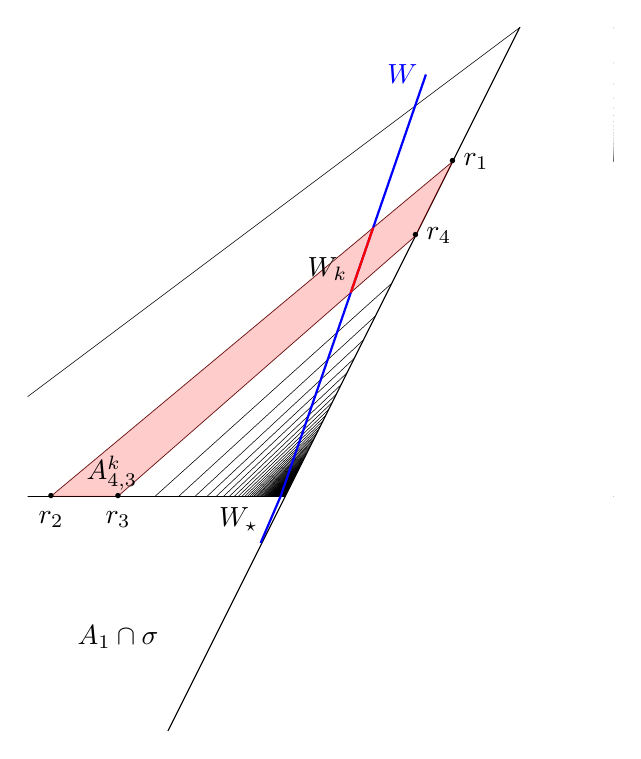
\begin{tikzpicture}[scale=0.85*7]
    
    \clip (1.95,4.5) rectangle (3.2,6);
    \foreach \k in {1,...,60}{
    \draw[very thin] ({ 5+ (2*\k+2)*(5-7.5)/(2*\k+1)  }, { 5 })--({ 5+ (2*\k+2)*(7.5-7.5)/(2*\k+1) }, { 7.5 });
    }
    

    
    \fill[black] (2.47,5) -- (2.53,5.06) -- (2.53,5) -- (2.47,5) ;
    \draw (0,5) -- (5,5);
    \filldraw[fill=white](0,0) -- (5,10) -- (5,0) -- (0,0);
    \draw [blue, thick] (1713/700,4.9) --(2.49,5)-- (2.8,5.9);
    \draw [red, thick] (6639/2515,5.4348) -- (739/275,613/110);
    
    \filldraw[red,fill=red,opacity=0.2] (2,5) -- (30/14,5) -- (50/18,50/9) -- (40/14,40/7) -- (2,5);
    \node at (2.13, 5.05) {$A_{4,3}^k$};
    \node at (6639/2515-0.05,5.4348+0.05) {$W_k$};
    \node at (2.4,4.95) {$W_\star$};
    \node at (2.75,5.9) {\color{blue}$W$\color{black}};

    \node[scale=0.5] at (2,5) {$\bullet$};
    \node at (2,4.95) {$r_2$};
    
    \node[scale=0.5] at (30/14,5) {$\bullet$};
     \node at (30/14,4.95) {$r_3$};
    \node[scale=0.5] at  (50/18,50/9) {$\bullet$};
     \node at (50/18+0.05,50/9) {$r_4$};
     \node[scale=0.5] at (40/14,40/7) {$\bullet$};
      \node at (40/14+0.05,40/7) {$r_1$};
    \node at (30/14,4.7) {$A_1 \cap \sigma$};

    \end{tikzpicture}
    }
    \subfigure[][]{
    \label{fig:twoStepB}
    \begin{tikzpicture}
    
    \node at (0,0) {
    \begin{tikzpicture}[scale=0.85*12]
    \clip (4.96,6.6) rectangle (5.35,7.7);
     \foreach \k in {1,...,80}{
        \draw({ 2.5 + (2*\k+1)*(5-5)/(2*\k)  }, { 5 })--({ 2.5 + (2*\k+1)*(10-5)/(2*\k)  }, { 10 });
    }
    \fill[fill=white] (5,10) -- (5,7.5) -- (10,10) -- (5,10);
    
    \node at (5.20,7.36) {$A_{1,3}^l$};
    
    \draw (5,7.5) -- (10,10);
   
    \filldraw[fill=white] (5,10) rectangle (4.8,5);
    
    \filldraw[red,fill=red,opacity=0.3] ({5+10/(4*8+2)},{7.5 - 50/(8*8+4) }) -- ({5+10/(4*8-2)},{7.5 - 50/(8*8-4) }) -- (5, {7.5 + 10/(8*8+4) } ) -- (5, {7.5 + 10/(8*8+12) } ) -- ({5+10/(4*8+2)},{7.5 - 50/(8*8+4) });
    
    %\node at (5.15,7.65) {$A_4 \cap \sigma$};
    
    \node[scale=0.5] at ({5+10/(4*8+2)},{7.5 - 50/(8*8+4) }) {$\bullet$};
     \node at ({5+10/(4*8+2) - 0.02},{7.5 - 50/(8*8+4) }) {$r_1'$};
    
    \node[scale=0.5] at ({5+10/(4*8-2)},{7.5 - 50/(8*8-4) }) {$\bullet$};
    \node at ({5+10/(4*8-2)-0.02},{7.5 - 50/(8*8-4) }) {$r_2'$};
    \node[scale=0.5] at  (5, {7.5 + 10/(8*8+4) } ) {$\bullet$};
    \node at (5+0.02, {7.5 + 10/(8*8+4) } ) {$r_3'$};
     \node[scale=0.5] at (5, {7.5 + 10/(8*8+12) } ) {$\bullet$};
    \node at (5-0.02, {7.5 + 10/(8*8+12) } ) {$r_4'$};
    
    \fill[fill=black] (5,7.48) -- (5,7.5) -- (5+0.03,7.5+0.015) -- (5,7.48);
    
    \end{tikzpicture}
    };

    \draw[dashed] (-0.4,1.4) circle (0.6cm);
    \draw[dashed] ({-0.4+0.6*cos(315)},{1.4+0.6*sin(315)}) -- ({2.6+2*cos(160)},{0.1+2*sin(160)});
    
    \filldraw[dashed, fill=white] (2.6,0.1) circle (2cm);
    
    \node[scale=1.5] at (2.6+1.05,-1.2) {\color{red}$U_{k}$\color{black}};
    
    \begin{scope}
    \clip (2.6,0.1) circle (2cm);
    \draw[thick]  ({2.6+2*cos(170)},{0.1+2*sin(170)}) -- ({2.6+2*cos(80)},{0.1+2*sin(80)});
    \draw[thick]  ({2.6+2*cos(250)},{0.1+2*sin(250)}) -- ({2.6+2*cos(-5)},{0.1+2*sin(-5)});
     
    \filldraw[red,fill=red,opacity=0.2] (1,2) -- (2.5,2.6) -- (4.5,-2.4) -- (3,-3) -- (1,2);
     
    \draw[red,very thick] ({2.6+2*cos(110)},{0.1+2*sin(110)}) -- ({2.6+2*cos(295)},{0.1+2*sin(295)});
    \draw[blue,very thick] ({2.6+1.48*cos(109)},{0.1+1.48*sin(109)}) -- ({2.6+1.24*cos(296.5)},{0.1+1.24*sin(296.5)});
    \node[scale=1.5] at (2.6+0.6,0.1+0.2) {\color{blue}$U_{k,l}$\color{black}};
    \end{scope}
    
    
    \end{tikzpicture}
    }
    
    
    
    \caption{Part (a) shows an unstable curve $W$ passing near to the accumulation point $(1/4,1/2)$, split into $W_\star$ below $y=1/2$ and the collection $W_k \subset A_{4,3}^k$. Part (b) shows the image $U_k = H_\sigma(W_k) \subset H_\sigma \left(A_{4,3}^k \right)$, which for odd $k$ lies near the accumulation point $(1/2,3/4)$ and contains subcurves $U_{k,l} \subset A_{1,3}^l$.}
    \label{fig:oneStep}
\end{figure}


\begin{prop}
\label{prop:upperTwoStep}
Condition (\ref{eq:oneStep}) holds for $H_\sigma^2$ when $W \cap B_\varepsilon(P_2) \neq \varnothing$ for all $\varepsilon>0$.
\end{prop}

\begin{proof}
We begin with the case $W \cap B_\varepsilon((1/4,1/2)) \neq \varnothing$ and let $\varepsilon \to 0$. We may choose $\delta$ sufficiently small so that $W$ intersects $A_1 \cap \sigma$ and some collection of sets $A_{4,3}^k$, $k_0 \leq k \leq k_1$, where $k_1 \to \infty$ as $\varepsilon \to 0$, $k_0 \to \infty$ as $\delta \to 0$. Therefore, $\mathcal{S}$ splits $W$ into a lower component $W_\star \subset A_1 \cap \sigma$ and upper components $W_k \subset A_{4,3}^k$, illustrated in Figure \ref{fig:twoStepA}. We study how the images of these components under $H_\sigma$ are split up by $\mathcal{S}$.

Recall the corners $r_j(k)$ which define $A_{4,3}^k$ near $(1/4,1/2)$. The curve $W_k$ has endpoints on $r_1r_2$ and $r_3r_4$, and all tangent vectors to $W$ lie in $\mathcal{C}_1$. For odd $k$ the image $U_k = H_\sigma(W_k)$ is a curve joining $r_1'r_2'$ to $r_3'r_4'$, with tangent vectors aligned in $M_4M_3^k \, \mathcal{C}_1$. This curve is split by $\mathcal{S}$ into an upper portion $U_{k,\star} \subset A_4 \cap \sigma$, and a collection $U_{k,l} \subset A_{1,3}^l$ for some consecutive range $l_0 \leq l \leq l_1$ which depends on $k$. Each $A_{1,3}^l$ is bounded by the lines
\begin{equation}
    \label{eq:linesLl}
    \mathcal{L}_l: y- \frac{1}{2} = \frac{2l}{2l+1} (x-1/4)
\end{equation}
and $\mathcal{L}_{l-1}$, hence a lower bound on $l_0(k)$ is given by the largest $l$ such that $r_2'(k)$ lies on or above $\mathcal{L}_{l-1}$. One can verify that $r_2'(k)$ lies on $\mathcal{L}_{l-1}$ when $k = 7l-4$ and approaches $(1/2,3/4)$ monotonically in $x$ and $y$ so that $l_0(k) \geq \lfloor \frac{k+4}{7} \rfloor$. To determine an upper bound on $l_1$, note that $r_4'r_1'$ lies on the line
\begin{equation}
    \label{eq:cellLinesk}
    y - \frac{3}{4} -\frac{1}{8k+12} = - \frac{6k+8}{2k+3} \left(x-\frac{1}{2} \right),
\end{equation}
meeting the $A_4$ boundary $\mathcal{L} : y=1/2 + x/2$ at the point
\begin{equation}
\label{eq:xkykonL}
    (x_k,y_k) =  \left( \frac{7k+10}{14k+19}, \frac{21k+29}{28k+38} \right).
\end{equation}
We similarly calculate that the line $\mathcal{L}_l$ meets $y=1/2 + x/2$ at the point
\[ (X_l,Y_l) = \left( \frac{l}{2l-1}, \frac{1-3l}{2-4l}  \right). \]
The intersection of $U_k$ with $y=1/2 + x/2$ must be some point $(x,1/2+x/2)$ with $x\geq x_k$ so that an upper bound on $l_1(k)$ is the smallest $l$ such that $x_k \geq X_l$, which reduces to $l \geq 7k+10$, hence $l_1(k) \leq \lceil 7k+10 \rceil = 7k+10$. For even $k$ the splitting behaviour is entirely analogous, with $H_\sigma(W_k)$ intersecting $\mathcal{S}$ in the neighbourhood of $(1,1/4)$.

For the lower component $W_\star$, the image $U_\star$ = $H_\sigma(W_\star) = H(W_\star)$ lies in a neighbourhood of $H(1/4,1/2) = (1/4,1)$ and is split by $\mathcal{S}$ into a collection $U_{\star,j} \subset A_{4,3}^j$, $j_0 \leq j \leq j_1$, where $j_1 \to \infty$ as $\varepsilon \to 0$, $j_0 \to \infty$ as $\delta \to 0$. Write $W_{\star,j} = H_\sigma^{-1}(U_{\star,j})$, $W_{k,\star} = H_\sigma^{-1}(U_{k,\star})$, $W_{k,l} = H_\sigma^{-1}(U_{k,l})$, then $W$ splits into components
\begin{equation}
    \label{eq:Wsplitting}
    W = \left( \bigcup_{j \geq j_0} W_{\star,j} \right) \cup \left( \bigcup_{k \geq k_0}  W_{k,\star} \right) \cup \left(  \bigcup_{k \geq k_0} \bigcup_{l=l_0}^{l_1} W_{k,l}  \right)
\end{equation}
on which $DH_\sigma^2$ is constant. Let $V_{i} = H_\sigma(U_i) = H_\sigma^2(W_i)$, then for $q=1/2$:
\begin{equation*}
\begin{split}
    \sum_i \left( \frac{|W|}{|V_i|}\right)^q \frac{|W_i|}{|W|} & = \sum_i \sqrt{ \frac{|W_i|}{|V_i|} } \sqrt{ \frac{|W_i|}{|W|}}\\
    & = \sum_{j \geq j_0}  \sqrt{ \frac{|W_{\star,j}|}{|V_{\star,j}|} } \sqrt{ \frac{|W_{\star,j}|}{|W|}} +  \sum_{k \geq k_0}         \sqrt{ \frac{|W_{k,\star}|}{|V_{k,\star}|} } \sqrt{ \frac{|W_{k,\star}|}{|W|}}   + \sum_{k \geq k_0} \sum_{l=l_0}^{l_1} \sqrt{ \frac{|W_{k,l}|}{|V_{k,l}|} } \sqrt{ \frac{|W_{k,l}|}{|W|}} \\
    & \leq \sum_{j \geq j_0}  \sqrt{ \frac{1}{\Lambda_{\star,j} }} \sqrt{ \frac{|W_{\star,j}|}{|W|}} +  \sum_{k \geq k_0}  \sqrt{\frac{1}{ \Lambda_{k,\star}}} \sqrt{ \frac{|W_{k,\star}|}{|W|}}   + \sum_{k \geq k_0} \sum_{l=l_0}^{l_1} \sqrt{\frac{1}{ \Lambda_{k,l}}} \sqrt{ \frac{|W_{k,l}|}{|W|}}
    \end{split}
\end{equation*}
by Lemma \ref{lemma:piecewiseApprox}, where $\Lambda_i$ is the minimum expansion factor of $DH_\sigma^2$ on $W_i$ over the cone $\mathcal{C}_1$. Define $W_\diamond = W \setminus W_\star$ and let $0\leq p \leq 1$ denote the proportion $|W_\diamond| = p\,|W|$, then
\begin{equation*}
\begin{split}
  \liminf_{\delta \to 0} \sup_{W: |W|< \delta}  \sum_i \left( \frac{|W|}{|V_i|}\right)^q \frac{|W_i|}{|W|} \leq \sup_{0 \leq p \leq 1} \Bigg( & \lim_{j_0 \to \infty}  \sum_{j \geq j_0}  \sqrt{ \frac{1}{\Lambda_{\star,j} }} \sqrt{ \frac{(1-p)|W_{\star,j}|}{|W_\star|}} \\
  & + \lim_{k_0 \to \infty} \sum_{k \geq k_0}  \sqrt{\frac{1}{ \Lambda_{k,\star}}} \sqrt{ \frac{p\,|W_{k,\star}|}{|W_\diamond|}} \\
  & + \lim_{k_0 \to \infty} \sum_{k \geq k_0} \sum_{l=l_0}^{l_1} \sqrt{\frac{1}{ \Lambda_{k,l}}} \sqrt{ \frac{p\,|W_{k,l}|}{|W_\diamond|}}\, \Bigg).
    \end{split}
\end{equation*}
We put upper bounds on each of these sums using lower bounds on the expansion factors $\Lambda_i$ and geometric bounds on the curves $U_i$ terminating on $\mathcal{S}$. We use asymptotic notation $f \sim g$ for functions $f,g$ if $f/g \to 1$, and write $f \lesssim g$ if there is some function $h$ such that $f \leq h \sim g$.

Starting with the first sum, $DH_\sigma^2$ is given by $M_4M_3^jM_1 = (-1)^j \left( \begin{smallmatrix} - 2 j - 3 & - 6 j - 8\\6 j + 8 & 18 j + 21  \end{smallmatrix} \right)$ on each component $W_{\star,j}$ with minimum expansion factors given by
\begin{equation}
    \label{eq:Lambdastarj}
    \begin{split}
         \Lambda_{\star,j} & = \inf_{7/3 \leq m \leq 3} \sqrt{ \frac{ \left( -2j-3 -6jm-8m \right)^2 + (6j+8 +18jm + 21)^2  }{1+m^2}}\\
         & \sim \inf_{7/3 \leq m \leq 3} \sqrt{ \frac{ \left( 2+6m \right)^2 + (6 +18m)^2}{1+m^2}} \,j = \frac{48 \sqrt{145}}{29} \,j := c_\star \,j.
    \end{split}
\end{equation}
Each curve $U_{\star,j}$ has tangent vectors in $M_1\mathcal{C}_1$ satisfying $41/17 \leq |v_2|/|v_1| \leq 17/7$, $v_1v_2 \geq 0$. For each $j>j_0$, $U_{\star,j}$ traverses $A_{4,3}^j$ so that (making a similar calculation to equation \ref{eq:sigma1bhk}) Lemma \ref{lemma:componentLength} gives
\begin{equation}
    \label{eq:Ustarj}
    \frac{ a_\star }{j^2} \lesssim |U_{\star,j}| \lesssim \frac{b_\star}{j^2}
\end{equation}
for $a_\star = \frac{13}{80} \sqrt{2}$, $b_\star = \frac{41}{192} \sqrt{1+ 17^2/41^2}$ (calculated in the appendix, section \ref{sec:upperCalculationsAppendix}). The upper bound also trivially holds for $j=j_0$. Let $\Lambda_1^+$, $\Lambda_1^-$ denote the maximum and minimum expansion factors of $M_1$ over $\mathcal{C}_1$, then
\[|W_\star| = \sum_{j\geq j_0} |W_{\star,j}| \geq \sum_{j\geq j_0} \frac{|U_{\star,j}|}{\Lambda_1^+} \gtrsim \frac{a_\star}{\Lambda_1^+} \sum_{j \geq j_0+1} \frac{1}{j^2} \geq \frac{a_\star}{\Lambda_1^+ (j_0+1)} \sim \frac{a_\star}{\Lambda_1^+ j_0}\]
where we have used the fact that
\[ \frac{1}{j^2} \geq \frac{1}{j(j+1)} = \frac{1}{j} - \frac{1}{j+1}\]
and considered the telescoping sum. Similarly $|W_{\star,j}| \lesssim b_\star / \left(\Lambda_1^- j^2 \right)$ so that
\[ \frac{|W_{\star,j}|}{|W_\star|} \lesssim \frac{b_\star \Lambda_1^+ j_0}{a_\star\Lambda_1^-} \, \frac{1}{j^2}.\]
Hence
\begin{equation}
\label{eq:Wstar}
    \begin{split}
        \sum_{j \geq j_0}  \sqrt{ \frac{1}{\Lambda_{\star,j} }} \sqrt{ \frac{(1-p)|W_{\star,j}|}{|W_\star|}} & \lesssim  \sum_{j \geq j_0} \sqrt{\frac{1}{c_\star j}} \sqrt{ \frac{(1-p)b_\star \Lambda_1^+ j_0}{a_\star\Lambda_1^-} \, \frac{1}{j^2} }\\
        & = \sqrt \frac{(1-p)b_\star \Lambda_1^+ j_0}{c_\star a_\star\Lambda_1^-} \sum_{j \geq j_0} j^{-3/2}\\
        & \leq \sqrt \frac{(1-p)b_\star \Lambda_1^+}{c_\star a_\star\Lambda_1^-} \, 2 \sqrt{\frac{j_0}{j_0-1}} \\
        & \to 2\sqrt \frac{(1-p)b_\star \Lambda_1^+}{c_\star a_\star\Lambda_1^-}
    \end{split}
\end{equation}
as $j_0 \to \infty$, where we have used $\sum_{j \geq j_0} j^{-3/2} \leq \int_{j_0-1}^\infty x^{-3/2} \d x$.

Moving onto the next summation, $\Lambda_{k,\star}$ is determined by $M_4^2M_3^k = (-1)^k \left( \begin{smallmatrix}  14 k + 5 & - 14 k - 12\\- 34 k - 12 & 34 k + 29 \end{smallmatrix} \right)$ and satisfies
\[ \Lambda_{k,\star} \sim \inf_{7/3 \leq m \leq 3} \sqrt{\frac{(14-14m)^2+(34-34m)^2}{1+m^2}} \, k = \frac{104}{\sqrt{29}}\, k =: c_\diamond \, k.\]
For odd $k$ the curve $U_{k,\star}$ has endpoints $(1/2,y_0)$ on $r_3'r_4'$ and $(2y_1-1,y_1)$ on $\mathcal{L}$, where $y_1$ is bounded by the intersections of $r_4'r_1'$ and $r_3'r_2'$ with $\mathcal{L}$ (see Figure \ref{fig:twoStepB}). An upper bound on $|y_1-y_0|$ is given by taking $(1/2,y_0) = r_3'$ and $(2y_1-1,y_1) = r_4'r_1' \cap \mathcal{L}$. Noting (\ref{eq:xkykonL}), this gives
\[ |y_1-y_0| \leq \frac{3}{4} + \frac{1}{8k+4} - \frac{21k+29}{28k+38} = \frac{6k+9}{56k^2+104k+38} \sim \frac{6}{56}k^{-1}. \]
$U_{k,\star}$ has tangent vectors $(v_1,v_2)^T$ in $M_{4,3}^k \, \mathcal{C}_1 \subset \mathcal{C}_4$, so that $|v_2/v_1| \geq 7/3$. By Lemma \ref{lemma:componentLength} we then have $|U_{k,\star}| \lesssim b_\diamond /k$, where $b_\diamond = \frac{6}{56} \sqrt{1 + \frac{9}{49}} \approx 0.117$. The minimum expansion factor of $M_4M_3^k = (-1)^k \left( \begin{smallmatrix}
  2k+1 & -2k-2\\
  -6k-2 & 6k+5
\end{smallmatrix}\right)$ over $\mathcal{C}_1$ is given by
\[\inf_{7/3 \leq m \leq 3} \sqrt{\frac{(2-2m)^2+(6-6m)^2}{1+m^2}} \, k = \frac{8\sqrt{145}}{29}\, k =: \gamma \, k\]
which gives $|W_{k,\star}| \lesssim b_\diamond/\left(\gamma k^2 \right)$. The analysis for even $k$ is analogous and gives the same upper bound. We next require a lower bound on $|W_\diamond|$. For $k>k_0$, $W_k$ is a curve with tangent vectors in $\mathcal{C}_1$ which traverses $A_{4,3}^k$. Making the same calculation as (\ref{eq:sigma1bhk}), $|W_k|$ is bounded below by the shortest path across $A_{4,3}^k$, the line segment passing through $r_4$ with gradient $3$. That's
\begin{equation}
\label{eq:Wklength}
    |W_k| \geq \sqrt{ \left( \frac{1}{16k^2+28k+6} \right)^2 + \left( \frac{3}{16k^2+28k+6} \right)^2 } \sim \frac{\sqrt{10}}{16k^2}
\end{equation}
so that 
\begin{equation}
\label{eq:Wdiamond}
    |W_\diamond| \geq \sum_{k\geq k_0+1} |W_k| \gtrsim \frac{a}{k_0}
\end{equation}
with $a:= \sqrt{10}/16$. Hence
\[\sum_{k \geq k_0}  \sqrt{\frac{1}{ \Lambda_{k,\star}}} \sqrt{ \frac{p\,|W_{k,\star}|}{|W_\diamond|}} \lesssim  \sum_{k \geq k_0} \sqrt{\frac{1}{c_\diamond k}} \sqrt{ \frac{p b_\diamond k_0}{a \gamma} \, \frac{1}{k^2} } \to 2\sqrt{\frac{pb_\diamond}{c_\diamond a \gamma}}\]
as $k_0 \to \infty$, by a similar argument to (\ref{eq:Wstar}).

For the third summation, $\Lambda_{k,l}$ is determined by the matrix \[M_1M_3^lM_4M_3^k = (-1)^{k+l} \begin{pmatrix} -48 k l - 10 k - 18 l - 3 & 48 k l + 10 k + 42 l + 8 \\ -112 k l - 26 k - 42 l - 8 & 112 k l + 26 k + 98 l + 21 \end{pmatrix}  \]
and satisfies (for large $k,l$)
\[ \Lambda_{k,l} \sim \inf_{7/3 \leq m \leq 3} \sqrt{\frac{(48-48m)^2+(112-112m)^2}{1+m^2}} \, kl = 64 \,kl =: c \,kl.\]
We can show an upper bound $|U_{k,l}| \lesssim b/l^2$ where $b = \frac{3}{32}\sqrt{1 + \frac{9}{49}} \approx 0.102$ (see section \ref{sec:upperCalculationsAppendix}) so that $|W_{k,l}| \lesssim b/(\gamma k l^2)$. Now by (\ref{eq:Wdiamond}),
\begin{equation*}
    \begin{split}
        \sum_{l=l_0}^{l_1} \sqrt{\frac{1}{ \Lambda_{k,l}}} \sqrt{ \frac{p|W_{k,l}|}{|W_\diamond|}} & \lesssim \sum_{l=l_0}^{l_1} \sqrt{\frac{1}{c\,kl}} \sqrt{\frac{p b k_0}{a \gamma k l^2}} \\
        & \leq \sqrt{\frac{1}{c\,k}} \sqrt{\frac{p b k_0}{a \gamma k}} \sum_{l=\lfloor \frac{k+4}{7} \rfloor}^{7k+10} l^{-3/2} \\
        & \leq 2 \sqrt{\frac{1}{c\,k}} \sqrt{\frac{p b k_0}{a \gamma k}} \left( \frac{1}{\sqrt{\lfloor \frac{k+4}{7} \rfloor -1}} - \frac{1}{\sqrt{7k+10}}   \right) \\
        & \sim 2 \sqrt{\frac{1}{c\,k}} \sqrt{\frac{p b k_0}{a \gamma k}} \left( \sqrt{7}- \frac{1}{\sqrt{7}} \right) \frac{1}{\sqrt{k}}.
    \end{split}
\end{equation*}
Letting $h = (\sqrt{7} - 1/\sqrt{7})^2 = 36/7$, we have that
\begin{equation*}
    \begin{split}
        \sum_{k \geq k_0} \sum_{l=l_0}^{l_1} \sqrt{\frac{1}{ \Lambda_{k,l}}} \sqrt{ \frac{p|W_{k,l}|}{|W_\diamond|}} & \lesssim 2 \sqrt{\frac{p b h k_0}{ca \gamma}}\sum_{k \geq k_0} k^{-3/2} \\
        & \to 4 \sqrt{\frac{p b h}{ca \gamma}}
    \end{split}
\end{equation*}
as $k_0 \to \infty$. Hence for $q=1/2$
\begin{equation}
    \label{eq:justConstants}
 \liminf_{\delta \to 0} \sup_{W: |W|< \delta}  \sum_i \left( \frac{|W|}{|V_i|}\right)^q \frac{|W_i|}{|W|} \leq \sup_{0 \leq p \leq 1} \left( 2\sqrt \frac{(1-p)b_\star \Lambda_1^+}{c_\star a_\star\Lambda_1^-} +    2\sqrt{\frac{pb_\diamond}{c_\diamond a \gamma}} +  4 \sqrt{\frac{p b h}{ca \gamma}} \right).
\end{equation}
It is simple to show that for $s,t>0$ the function $f(p) = s\sqrt{1-p} + t\sqrt{p}$ always attains its maximum value at $p = t^2/(s^2+t^2)$. Hence letting
\[ s =  2\sqrt \frac{b_\star \Lambda_1^+}{c_\star a_\star\Lambda_1^-} \approx 0.450, \quad t = 2\sqrt{\frac{b_\diamond}{c_\diamond a \gamma}} +  4 \sqrt{\frac{ b h}{ca \gamma}} \approx 0.639 \]
gives
\[ \liminf_{\delta \to 0} \sup_{W: |W|< \delta}  \sum_i \left( \frac{|W|}{|V_i|}\right)^q \frac{|W_i|}{|W|} \leq s\sqrt{\frac{s^2}{s^2+t^2}} + t\sqrt{\frac{t^2}{s^2+t^2}} \approx 0.781 < 1  \]
as required. The analysis is analogous for $W$ near $(1/4,1)$ and extends to $W$ near $(3/4,0)$ and $(3/4,1/2)$ using the symmetry $T(x,y) = (1-x,y+1/2)$ which commutes with $H_\sigma$ (as seen in the proof of Lemma \ref{lemma:unstableGrowth}).
\end{proof}

Equivalent analysis verifies the two step expansion for curves near the other accumulation points $p \in P_1$. We provide the relevant calculations to the appendix, Proposition \ref{prop:lowerTwoStep}. We are now ready to apply Theorem \ref{thm:chernovZhang}.

\subsection{Decay of correlations}

\begin{thm}
\label{thm:HsigmaExp}
The return map $H_\sigma: \sigma \to \sigma$ enjoys exponential decay of correlations. In particular it admits a Young tower with base $\Delta_0$ satisfying the exponential tail bound
\begin{equation}
    \label{eq:delta0tailbound}
    \mu\left( \{ z \in \sigma \, | \, R(z,H_\sigma,\Delta_0) > n \} \right) \leq \mathrm{const} \, \theta^n
\end{equation}
for all $n \geq 1$ where $\theta<1$ is some constant. 
\end{thm}

\begin{proof}

We run through the conditions for applying Theorem \ref{thm:chernovZhang}. Invariance of the unstable and stable cone fields $C_z^u$, $C_z^s$ was the subject of section \ref{sec:invariantCones}, satisfying \textbf{(H1.1)}. Condition \textbf{(H1.2)} follows by taking $\Lambda = \sqrt{85/41}$, with this lower bound attained by considering the expansion of $M_2^{-1}$ over the cone boundary of $\mathcal{C}_2^s$ with gradient $-8/10$. Noting Remark \ref{remark:firstRemark}, we next show \textbf{(H1.3')}. The cone fields are continuous over the components $\sigma_j$ of $\Omega \setminus \mathcal{S}_0$, indeed they are constant. Noting that all of the stable cones lie within $\mathcal{C}_1^s$ and all of the unstable cones lie in $\mathcal{C}$, a positive angle between stable and unstable cone fields follows from $\mathcal{C}_1^s \cap \mathcal{C} = \varnothing$. \textbf{(H2)} was the subject of section \ref{sec:singSetStructure}. Unstable manifolds provide a class of $H_\sigma$ invariant unstable curves which satisfy the regularity conditions listed in \cite{chernov_statistical_2009}. Piecewise linearity of the map trivially implies their bounded curvature and bounds on distortion; absolute continuity follows from Lemma \ref{lemma:HsigmaKatokStrelcyn}. \textbf{(H4)} follows from Proposition \ref{prop:HsigmaBernoulli}, where we showed that $H_\sigma$ is Bernoulli with respect to the normalised Lebesgue measure on $\sigma$. Noting Remark \ref{remark:firstRemark}, \textbf{(H5)} follows for the map $H_\sigma^2$ by Propositions \ref{prop:simple2step}, \ref{prop:upperTwoStep}, \ref{prop:lowerTwoStep}.
\end{proof}

